\chapter{The Runtime Library} \label{chp:runtime}
\section{Introduction} \label{sec:runtime/introduction}
In this chapter, the work performed towards implementing the runtime library, known as Locomotion, is presented. This library handles several core functions critical to the infrastructure of the application:

\begin{itemize}
	\item Functions for collecting trace analyses
	\item Implementations of trace storage backends
	\item Algorithms for offline and online dependency analysis
\end{itemize}

The programs described within this chapter are open-source, released under The University of Edinburgh GPL license. They are available at \url{https://github.com/chrisatkin/locomotion}.

The fully-qualified package identifier for the runtime library is\\\texttt{uk.ac.ed.inf.icsa.locomotion.instrumentation}.

\section{Trace Storage} \label{sec:runtime/storage}
Generating traces for large programs -- the kind of programs which would benefit from hot-loop analysis -- requires a large amount of storage as it scales linearly with the number of memory operations ($S=O(n)$). Although the number of storage operations conforming to the requirements in a program may be relatively small, this number is increased when the standard library is included.

The main problem that the storage format must be able to determine is this. Given trace $T$ and access $\alpha$, is $\alpha \in T$?
	
	\subsection{Exact Approaches} \label{sec:runtime/storage/exact}
	Exact approaches provide an accurate deterministic response to this question. They are not probabilistic or statistical in nature.
	
		\subsubsection{Hash Tables and Sets} \label{sec:runtime/storage/exact/hashing}
		A hash function maps keys to indexes, where buckets are stored. Buckets contain all items with the same key. Ideally, a lookup of $T=O(1)$ is possible (\ie, a hash function with ideal distribution). Worst-case cost is $T=O(n)$, in the case of multiple collisions or a low load factor, as the bucket will need to be traversed sequentially to find the item.
		
		It is common to use hashing by division for the hash function:
		
		\[
			f(k) = k \bmod{D}
		\]
		
		Where $k$ is the key and $D$ is the size (\ie, number of positions of the hash table) \citep{DSandAlgsCpp}.
		
		The constant-time lookup assumes that the \textit{load factor} $L$ is bounded below some constant. The load factor is computed by $L=\frac{n}{k}$.
		
		Figure \ref{fig:hash-table} demonstrates a simple hash table without collisions.
		
		\begin{figure}
			\centering
			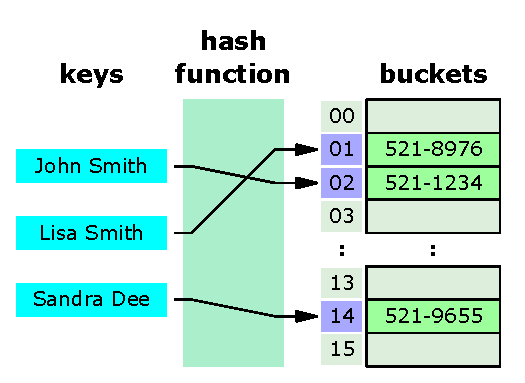
\includegraphics[width=0.7\textwidth]{graphics/hash-table.pdf}
			\caption{A simple hash table for a phone book}
			\label{fig:hash-table}
		\end{figure}

	\subsection{Probabilistic Approaches} \label{sec:runtime/storage/probabilistic}
	The main disadvantage to using exact approaches is that the storage required scales linearly such that $S=O(n)$. For anything but the most trivial programs, this means that it becomes infeasible to store traces for all memory operations.
	
		\subsubsection{Bloom Filters} \label{sec:runtime/storage/probabilistic/bloom}
		One alternative is the use of Bloom Filters \citep{Bloom1970}. A Bloom Filter is a randomised data structure which supports membership queries, with the possibility of false positives. In the context of parallelism detection, this means that we may conclude that a loop is not parallelisable when in reality, it is.
		
		The operation of a Bloom Filter is simple: there exists a bit vector of size $m$ and a number $k$ of hash functions (which could use universal hashing \citep{Carter1979}). Upon insertation of an item $i$, for each hash $k_n$ the value of $v_n=k_n(i)$ is computed, which is an integer in the range $0..m$. The corresponding index of the vector is then set to $1$.
		
		\begin{figure}[h!]
				\centering
				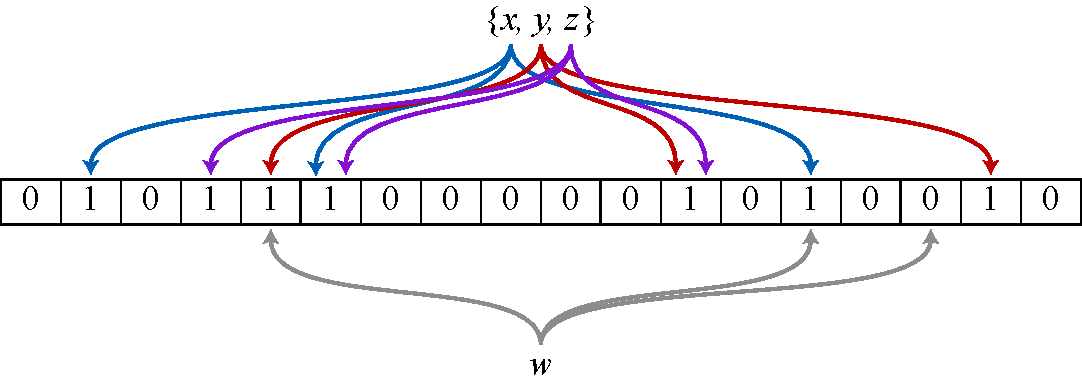
\includegraphics[width=0.8\textwidth]{graphics/bloomfilter.pdf}
				\caption{Bloom filter operation with $m=18$ and $k=3$}
				\label{fig:bloom-filter}
		\end{figure}
			
		To test membership for an item, feed the item to each hash function. If all the corresponding indexes are $1$, then the item \emph{may} be contained within the filter - if any of them are $0$, then the item is definitely not.
		
		For a given number of entries $s$ and a bit vector of size $m$, we need to use $k$ hash functions such that:
		
		\begin{equation}
			k = \frac{m}{s} \ln 2
			\label{eqn:optimal-hashes}
		\end{equation}
		
		The error rate is defined as:
		
		\[
		\sigma = 0.5^k
		\]
		
		In essence, the longer the bit vector, the more accurate the filter becomes - at the expense of increasing space requirements. If $m=\infty$, then there are no false positives - the filter becomes accurate and deterministic (for a fixed set of $k$).
		
		\citet{Swamidass2007} show is that the number of elements within a Bloom Filter can be estimated by:
		
		\[
		E = -n \ln \frac{1-n/n}{k}
		\]
		
		% return (long) (-n * Math.log(p) / (Math.log(2) * Math.log(2)));
		
		It is possible to calculate the theoretical optimal length of the bit vector $m$ from the number of expected insertions $n$ and the \textit{false positive rate} $p$. This is defined as

		\[
			m = -n \times \log(p) \div \log(2) \times \log(2)
		\]
		
		The main advantage of bloom filters is that the space complexity is constant $S=O(c)$, where $c$ is the size of the bit vector. This will allow memory overhead to be substantially lower, whilst still retaining $T=O(1)$ lookup time complexity. As mentioned above, this is a significant (factor $n$) improvement over the exact approach.
		
		However, lookup time in bloom filters is asymptotically greater than the hash-based alternative. Unlike the hashing-based approach which has, with an optimal load factor, a lookup time of $T_{lookup}^{hash}=O(1)$, a bloom filter has a lookup time of $T_{lookup}^{bloom}=O(k)$ (where $k$ is the number of hash functions). This is unlike amongst array/vector-based approaches, which in many cases are $T=O(1)$. As the number of optimal hash functions is dependent on the number of expected entries and the bit vector size (see equation \ref{eqn:optimal-hashes}), it is predicted that execution time will increase slightly as a result, with the assumption that the hashing-based approach is operating efficiently (\ie, with an adequate load factor).
		
		We hypothesise that, with the correct parameters, it is possible to effectively use probabilistic approaches in order to reduce both the memory and execution time overhead associated with dependency analysis.

\section{Dependency Analysis Algorithms} \label{sec:runtime/analysis}
	Computing dependency between two operations is of critical importance to this project; an efficient algorithm is important.
	
	From \citet[p.~37]{Allen2000}, there is a data dependence from statement $\sigma_x$ to statement $\sigma_y$ (where $T(\sigma_x) \rightarrow T(\sigma_y)$\footnote{For two statements $x$ and $y$, $x \rightarrow y$ iff $T(x) < T(y)$ where $T(e)$ returns the time at which $e$ occured}) if and only if:
	
	\begin{enumerate}
		\item both statements access the same memory location and at least one of them stores into it
		\item there is a feasible run-time execution path from $\sigma_x$ to $\sigma_y$
	\end{enumerate}
	
	There are several kinds of inter-iteration dependency \citep[p.~526]{Ibbett2009,ArchitectureBook}:
	
	\begin{itemize}\label{fig:dep-kinds}
		\item \textbf{Write-after-write} or \textit{output dependency}: given two statements $\sigma_x$ and $\sigma_y$, there is a write-after-write dependency if a total ordering is required for $\sigma_x$ and $\sigma_y$. For example:
		
		\begin{verbatim}
		R3 = R1 + R2
		R3 = R3 + R4
		\end{verbatim}
		
		If the second statement were executed before the first statement, program correctness would be violated, so speculative execution is not possible.
		
		Output dependence for two statements $\sigma_x$ and $\sigma_y$ is denoted as $\sigma_x \delta^0 \sigma_y$.
		
		\item \textbf{Write-after-read} or \textit{antidependency}: given two statements $\sigma_x$ and $\sigma_y$, there is a write-after-read dependency if evaluation of $\sigma_y$ is dependent on the evaluation of $\sigma_x$:
		
		\begin{verbatim}
		R1 = R2 + R3
		R2 = R4 + R5
		\end{verbatim}
		
		In this case, if the statements are re-ordered, the wrong value of \texttt{R2} will be used.
		
		Antidependence for two statements $\sigma_x$ and $\sigma_y$ is denoted as $\sigma_x \delta^{-1} \sigma_y$.
		
		\item \textbf{Read-after-write} or \textit{true dependency}: given two statements $\sigma_x$ and $\sigma_y$, there is a read-after-write dependency if $\sigma_y$ stores the value (or derivative value) of $\sigma_x$:
		
		\begin{verbatim}
		R1 = R2 + R3
		R4 = R1 + R5
		\end{verbatim}
		
		If the statements are reordered, either a stale value of R1 will be used, or R1 may not have been initialized.
		
		True dependency for two statements $\sigma_x$ and $\sigma_y$ is denoted as $\sigma_x \delta \sigma_y$.
	\end{itemize}
	
	There is also a theoretical dependency that can be detected by the framework, read-after-read, but since this does not cause two iterations to be dependent, they are not considered by the framework.
	
	For an arbitrary loop in which the loop index $I$ runs from $L$ to $U$ in steps of $S$, the iteration number $i$ of a specific iteration is equal to the value $\frac{I-L+S}{S}$, were $I$ is the value of the index on that iteration.
	
	Given a nest of $n$ loops, the \textit{iteration vector} $i$ of a particular iteration of the inner-most loop is a vector of integers that contain the iteration numbers for each of the loops in order of nesting level. $i$ is given by $i=\{i_1, i_2, ..., i_n\}$ where $ik$, $1 \leq k \leq n$, represents the iteration number for the loop at level $k$.
	
	There exists a loop dependence from statement $\sigma_1$ to $\sigma_2$ in a common next of loops iff there exists two iteration vectors $i$ and $j$ for the nets, such that:
	
	\begin{enumerate}
		\item $i < j \lor i = j$ and there is an execution path from $\sigma_x$ to $\sigma_y$ in the body of the loop
		\item Statement $\sigma_x$ accesses memory location $m$ on iteration $i$ (access $\alpha_x$) and statement $\sigma_y$ accesses location $m$ on iteration $j$ (access $\alpha_y$)
		\item Either $\alpha_x$ or $\alpha_y$ is a store
	\end{enumerate}
	
	Thus, the following problem declaration can be constructed for computing dependencies:
	
	Let $i^l_n$ be the set of memory accesses for iteration $n$ in loop $l$. For a memory access $\alpha \in i^l_n$, determine whether there exists a previous iteration such that $\alpha \in i^l_{n-c}$ for some integer $c$. Additionally, for an access $\alpha_i$ and previous access $\alpha_{i-c}$, $kind(\alpha_i) \neq read \land kind(\alpha_{i-c}) \neq read$.
	
	In addition, there are two kinds of loop dependence.
	
	\begin{itemize}
		\item \textbf{Loop-carried dependence}: $\sigma_x$ can reference a common location $m_c$ on an iteration, $\sigma_y$ can reference the same location $m_c$
		\item \textbf{Loop-independent dependence}: $\sigma_x$ and $\sigma_y$ can both access $m_c$ on the same iteration, but with $\sigma_x$ preceding $\sigma_y$ during execution
	\end{itemize}

	\subsection{Offline Algorithms} \label{sec:runtime/analysis/offline}
	An offline algorithm means that any processing is performed after the trace has been collected \citep[p.~525-526]{TAOCPvol2}. It is the simplest form of dependency analysis algorithm, but it show poor performance. For a number of loops $l$ with an average of $i$ iterations each, where each iteration has an average of $o$ operations, then $T_{offline}=O(lio)$.
	
	\begin{algorithm}
		\caption{Offline dependency algorithm}
		\label{alg:offline-dependency}
		\begin{algorithmic}[1]
			\STATE $d \gets \varnothing$ %\COMMENT{$d$ is the set of dependencies}
			\FORALL{loops $l$}
				\STATE $p \gets \varnothing$ %\COMMENT{$p$ is the set of previous iterations}
				\FORALL{iteration $i \in l$}
					\FORALL{access $\alpha \in i$}
						\FORALL{$p_{\alpha} \in p$}
							\IF{$\alpha \in p{_\alpha}$}
								\STATE $d \gets \alpha$
							\ENDIF
							
							\STATE $p \gets \alpha$
						\ENDFOR
					\ENDFOR
				\ENDFOR
			\ENDFOR
		\end{algorithmic}
	\end{algorithm}
	
	This offline algorithm has several disadvantages. Not only is its runtime particularly poor (we can achieve at least a factor $l$ speed-up using an online algorithm), but because it requires a complete trace of accesses per iteration, it is unsuitable for  detecting dependencies at run-time. Algorithm \ref{alg:offline-dependency} outlines the offline algorithm.

	\subsection{Online Algorithns} \label{sec:runtime/analysis/online}
	\begin{figure}
			\centering
			\begin{tikzpicture}[->,>=stealth',shorten >=1pt,auto,node distance=3.5cm,semithick, bend angle=35]
				\node[initial,accepting,state]	(q1)					{$S$};
				\node[state]					(q2)	[right of=q1]	{$Q$};
				
				\path[->]
					(q1)	edge [bend left ] node {loop begin} (q2)
					(q2)	edge [bend left] node {loop stop} (q1)
							edge [loop right] node {iteration} (q2);
					
			\end{tikzpicture}
			\caption{Finite state machine for the online algorithm}
			\label{fig:online-fsm}
		\end{figure}
		
	An online algorithm for this problem is one that runs with a sequential input of values. An online algorithm is superior because it shows better performance characteristics asymptotically, $T_{online} = O(io)$, and it runs in conjunction with the program. This allows Locomotion, in theory, to advice any JIT compilers of optimisations to perform. Figure \ref{fig:online-fsm} represents the finite state machine for the algorithm.
	
	\begin{algorithm}
		\caption{Online dependency algorithm}
		\label{alg:online-dependency}
		\begin{algorithmic}
			\STATE $d \gets \varnothing$ %\COMMENT{$d$ is the set of dependencies}
						\FORALL{loops $l$}
							\STATE $p \gets \varnothing$ %\COMMENT{$p$ is the set of previous iterations}
							\FORALL{iteration $i \in l$}
								\FORALL{access $\alpha \in i$}
									\FORALL{$p_{\alpha} \in p$}
										\IF{$\alpha \in p{_\alpha}$}
											\STATE $d \gets \alpha$
										\ENDIF
										
										\STATE $p \gets \alpha$
									\ENDFOR
								\ENDFOR
							\ENDFOR
						\ENDFOR
		\end{algorithmic}
	\end{algorithm}

\section{Implementation Details} \label{sec:runtime/implementation}
In this section, we consider the techniques used to implement the runtime library and online dependency algorithm from a software engineering perspective.

	\subsection{Entry Point} \label{sec:runtime/implementation/entry-point}
	The main entry point to the instrumentation is the \texttt{InstrumentSupport} class. It includes an \texttt{Instrument}, which is an implementation of instrumentation. There is also a number of static methods for accessing the instrumentation framework, such as starting and ending timers (and getting time differences in nanoseconds) and flushing the instrument buffers. Figure \ref{fig:instrument-support} shows the class diagram with public methods for \texttt{InstrumentSupport}.
	
	\begin{figure}
		\centering
		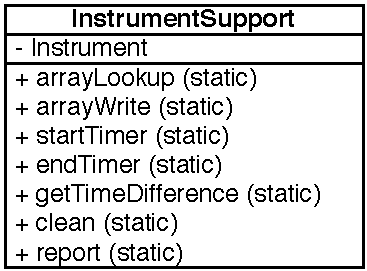
\includegraphics[width=0.4\textwidth]{graphics/instrument-support.pdf}
		\caption{Class diagram for \texttt{InstrumentSupport}}
		\label{fig:instrument-support}
	\end{figure}
	
	\subsection{Instrument Implementation} \label{sec:runtime/implementation/instrument}
	\texttt{InstrumentSupport} is initalised at load-time with an \texttt{Instrument} (via static blocks). \texttt{Instrument} is an implementation of instrumentation, and it has a configuration. This configuration contains parameters such as whether the instrumentation should be enabled and so on.
	
	The user-facing methods for trace collection have the following signatures:
	
	\begin{lstlisting}[caption=Method signatures for instrumentation methods,label=lst:sigs]
	public static <T> void
	arrayLookup(T[] array, int index, int i, int id);
	
	public static <T> void
	arrayStore(T[] array, int index, T value, int i, int id);\end{lstlisting}
	
	The arguments are:
	
	\begin{itemize} \label{items:trace-args}
		\item \texttt{T[] array}: the array upon which the operation is occuring
		\item \texttt{int index}: the array index in question
		\item \texttt{int i}: the value of the iteration variable
		\item \texttt{T value}: the value being written to the array at the index
		\item \texttt{int id}: a unique loop identifier
	\end{itemize}
	
	The Java generics system was leveraged in order to reduce the amount of code required to implement the collection; it is important to recognise that the Java type system allows the trace collection mechanism to be unconcerned with the type of the array being accessed (and the type of the item being inserted if appropriate).
	
	Although it would be possible to use the above generics-based methods for all data types, this would require the use of the object-oriented wrapper libraries (also called the reference types) for \texttt{int} $\rightarrow$ \texttt{Integer}, \texttt{float} $\rightarrow$ \texttt{Float} and so on. This would have the disadvantage of incurring the overhead of autoboxing \citep{boxing} in the library.
	
		\subsubsection{Java Auto(un)boxing} \label{sec:runtime/implementation/instrument/boxing}
		Despite being an object-oriented language, Java has several non-object-oriented types. These are known as \textit{primitive values}. They are not part of the standard object-hierarchy, and no methods can be called upon them. The primitive types are \texttt{int}, \texttt{long}, \texttt{char}, \texttt{float}, \texttt{double}, \texttt{boolean} and \texttt{short}.
		
		Unlike in C\# which has a \textit{unified type system} -- where \emph{all} types inherit from a single objct, regardless of being value/primitive types or reference types -- Java does not. Each primitive type has a corresponding reference type (named as such because Java uses pass-by-reference for objects), which is an object and hence part of the class hierarchy. Indeed, in C\# the `short names' for value types are actually aliases for the full identifiers, such as \texttt{System.Byte}, \texttt{System.Int32} and so on.
		
		Although this approach does have some advantages -- primitive types require less over head than the object-oriented value types -- there are some disadvantages. The Java compiler will automatically perform transformations on instances where:
		
		\begin{itemize}
			\item An identifier for a primitive type is passed where an identifier for a reference type is required or vica-versa
			\item \textbf{And} there is not a type error (so \texttt{int} cannot be transformed to \texttt{short})
		\end{itemize}
		
		This process is called auto boxing (in the case of primitive-to-reference type occurs) or auto unboxing (where reference-to-primitive type occurs). The advantage of this approach is that it simplifies programming and reduces `crufty' code. For example, adding two \texttt{Integer}, \texttt{a} and \texttt{b} doesn't require \texttt{Integer c = a.add(b);}, but instead the more natural \texttt{Integer c = a + b} can be used. In this case, \texttt{a} and \texttt{b} will be auto-unboxed to primitive types, the addition is performed and the result is autoboxed back to \texttt{Integer}.
		
		However, this automatic casting operation does occur a slight performance overhead, both in terms of memory and execution time. Although in most cases the overheads are small, for benchmarking a runtime system with somewhat significant overheads, another solution was opted for. Instead of only supporting value types, we \emph{also} support primitive types by overloading the appropriate methods. 
	
	\subsection{Trace Storage and Configuration} \label{sec:runtime/implementation/trace}
	The instrumentation includes implementations of both exact and inexact approaches to trace storage.
	
	The \texttt{Access} class provides an abstraction for an access. An \texttt{Access} represents an array access with an associated kind, index, number (``\textit{this iteration represents the $n$th access this iteration''}).
	
		\subsubsection{Exact - Hash Set} \label{sec:runtime/implementation/trace/hashset}
		For the exact implementation, I chose to use the standard Java Collections Framework \texttt{HashSet} class. This is for several reasons, such as:
		
		\begin{itemize}
			\item \textbf{Performance}: array lookup in hash maps is $T=O(1)$, assuming an equal distribution of hash codes. For this reason, \texttt{Access} also overrides the standard \texttt{hashCode()} implementation, so that any two accesses are equivalent iff the array ID and indexes match.
			
			\item \textbf{Uniform interface}: any member of the Collections framework includes by-default various capabilities, such as being \texttt{Iterable}, meaning enhanced for-each loops can be used.
			
			\item \textbf{Standard implementation}: the built-in implementation has been tested for bugs, and is (mostly) bug-free. A custom implementation could not be subjected to this same rigorous testing.
		\end{itemize}
		
		\subsubsection{Inexact - Bloom Filters} \label{sec:runtime/implementation/trace/bloom}
			Rather than creating a custom implementation of Bloom filters, I used an existing implementation in the form of Google Guava \citep{GuavaBloomFilter}.\
		
		There is a parent abstract class, \texttt{Trace} which specifies several standard methods that all interfaces must define (\texttt{add()}, \texttt{contains()} and \texttt{size()}). All implementations of traces inherit from this superclass. Figure \ref{fig:trace-classes} shows this hierarchy in detail.
		
		\begin{figure}
			\centering
			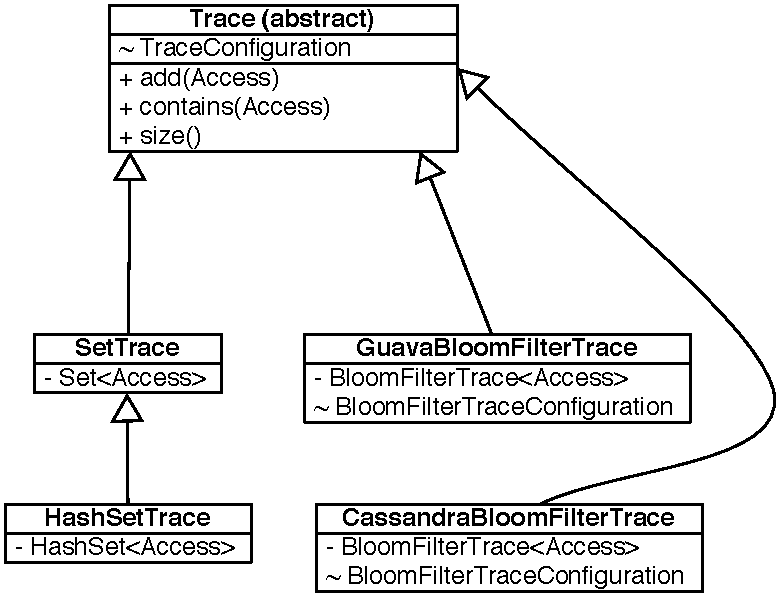
\includegraphics[width=0.7\textwidth]{graphics/trace-classes.pdf}
			\caption{Trace class hierarchy}
			\label{fig:trace-classes}
		\end{figure}
		
		A \texttt{TraceConfiguration} class is used to provide configuration details for the trace. There are no configuration variables used for hash sets, but for bloom filters this includes the initial size and the \texttt{Filter} used (an implementation detail as a result of the use of Google Guava). Dynamic configuration was preferred to constants as many experiments will need to be run, often with different variables.
		
		When a new access $\alpha$ in iteration $i$ and loop $l$ is detected, the library checks if $l$ is a new loop, or an existing one. If the loop is new, it instantiates a new \texttt{Loop} object, which holds the traces, as well as detecting whether an access is dependent. \texttt{Loop} stores two instantiations of the supplies \texttt{Trace} class - one for read and one for write operations. This is necessary in order to detect $\sigma_x \delta \sigma_y$, $\sigma_x \delta^0 \sigma_y$ and $\sigma_x \delta^{-1} \sigma_y$ dependencies, but not read-after-read dependencies. In order to use a single trace implementation, the semantics of the \texttt{hashCode()} and \texttt{equals()} methods, along with the \texttt{Comparable} access would need to be violated as a temporal dependence is introduced. Both bloom filters use \texttt{hashCode()} to determine an item is contained. It is not possible to use a $\sigma_x \delta \sigma_y$, $\sigma_x \delta^0 \sigma_y$ and $\sigma_x \delta^{-1} \sigma_y$ but not read-after-read dependencies.
		
		In order to detect dependencies, \texttt{Loop} checks all \emph{previous} iterations, using a $T=O(1)$ check on for containment within both read and write traces. Overall, for $n$ iterations the solution has a time complexity $T=O(n)$ and a space complexity $S=O(a)$, where $a$ is the number of accesses. Once a loop has been completed as detected by the finite state machine (see figure \ref{fig:online-fsm}), the accesses are deleted in order to reduce memory location.
		
		Dependencies are reported to the runtime via an exceptions mechanism. When a dependence is detected a special exception, \texttt{LoopDependencyException} is thrown, which is initialised with hazard metadata (which access is dependent, the kind of dependence, and the two iterations which the access occurs within). \texttt{LoopDependencyException} is a checked exception. The exception traverses up the stack until it reaches \texttt{Instrument}, which stores all exceptions of the same type in a linked list. This list is available to users of the framework, meaning full dependency information is available.

\section{Summary} \label{sec:runtime/summary}
In this chapter, the theory of dependence analysis has been introduced, as well as some practical approaches to implementing them. Both kinds of dependency checking algorithm (offline and online) have been covered, as well as implementation details of online algorithms in our framework.

Lastly, a software engineering-based approach to the design of the instrumentation framework was discussed.